% Chapter 10, Section 6

\section{Advanced Topics \difficultyInline{intermediate}}
\label{sec:rnn-advanced}

\subsection*{Intuition}

Variants extend context (bidirectional), depth (stacked layers), supervision signals (teacher forcing), and search quality (beam search). These choices trade training stability, inference latency, and quality depending on the task.

\subsection*{Historical Context}

Bidirectional RNNs improved context use for labeling tasks; teacher forcing stabilized decoder training but highlighted exposure bias; beam search became standard for autoregressive decoding in translation and speech.

% Index and glossary
\index{bidirectional RNN}
\index{teacher forcing}
\index{beam search}
\glsadd{attention-mechanism}

\subsection{Bidirectional RNNs}

Process sequence in both directions:
\begin{align}
\overrightarrow{\vect{h}}_t &= f(\vect{x}_t, \overrightarrow{\vect{h}}_{t-1}) \\
\overleftarrow{\vect{h}}_t &= f(\vect{x}_t, \overleftarrow{\vect{h}}_{t+1}) \\
\vect{h}_t &= [\overrightarrow{\vect{h}}_t; \overleftarrow{\vect{h}}_t]
\end{align}

Useful when future context is available.

\paragraph{Use cases and caveats.} Effective for tagging, chunking, and ASR with full utterances, but not suitable for strictly causal, low-latency streaming since backward states require future tokens. Alternatives include limited-lookahead or online approximations.

\subsection{Deep RNNs}

Stack multiple RNN layers:
\begin{equation}
\vect{h}_t^{(l)} = f(\vect{h}_t^{(l-1)}, \vect{h}_{t-1}^{(l)})
\end{equation}

Each layer captures different levels of abstraction.

\paragraph{Visual aid.} Stacked recurrent layers over time.
\begin{figure}[h]
    \centering
    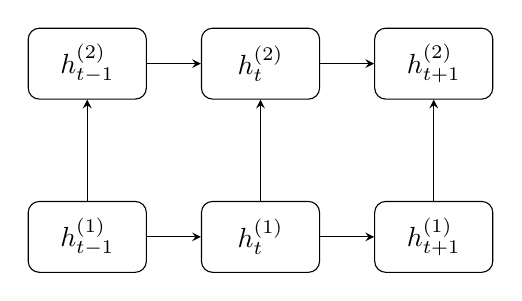
\begin{tikzpicture}[>=stealth, node distance=2.2cm]
        \tikzstyle{node}=[draw, rounded corners, minimum width=1.5cm, minimum height=0.9cm]
        % time t-1
        \node[node] (l1t1) {$\vect{h}_{t-1}^{(1)}$};
        \node[node, above of=l1t1] (l2t1) {$\vect{h}_{t-1}^{(2)}$};
        % time t
        \node[node, right of=l1t1] (l1t) {$\vect{h}_{t}^{(1)}$};
        \node[node, above of=l1t] (l2t) {$\vect{h}_{t}^{(2)}$};
        % time t+1
        \node[node, right of=l1t] (l1t2) {$\vect{h}_{t+1}^{(1)}$};
        \node[node, above of=l1t2] (l2t2) {$\vect{h}_{t+1}^{(2)}$};
        % horizontal
        \draw[->] (l1t1) -- (l1t);
        \draw[->] (l1t) -- (l1t2);
        \draw[->] (l2t1) -- (l2t);
        \draw[->] (l2t) -- (l2t2);
        % vertical
        \draw[->] (l1t1) -- (l2t1);
        \draw[->] (l1t) -- (l2t);
        \draw[->] (l1t2) -- (l2t2);
    \end{tikzpicture}
    \caption{Deep RNN: multiple recurrent layers stacked over time.}
\end{figure}

Practical tips: residual connections, layer normalization, and dropout between layers help optimization and generalization.

\subsection{Teacher Forcing}

During training, use ground truth as decoder input (not model's prediction):
\begin{itemize}
    \item Faster convergence
    \item Stable training
    \item May cause exposure bias at test time
    \;—a train–test mismatch where the model never learns to recover from its own errors. Mitigations include scheduled sampling and sequence-level training.
\glsadd{backpropagation}
\end{itemize}

\subsection{Beam Search}

For inference, maintain top-$k$ hypotheses:
\begin{itemize}
    \item Better than greedy decoding
    \item Trade-off between quality and speed
    \item Common beam size: 5–10; length normalization and coverage penalties are often used in NMT.
\end{itemize}
